%%%%%%%%%%%%  Generated using docx2latex.com  %%%%%%%%%%%%%%

%%%%%%%%%%%%  v2.0.0-beta  %%%%%%%%%%%%%%
% \documentclass[soumission]{ir} % Pour une soumission anonyme

\documentclass[12pt]{report}
\usepackage{amsmath}
\usepackage{latexsym}
\usepackage{amsfonts}
\usepackage[normalem]{ulem}
\usepackage{array}
\usepackage{amssymb}
\usepackage{graphicx}
\usepackage[backend=biber,
style=numeric,
sorting=none,
isbn=false,
doi=false,
url=false,
]{biblatex}\addbibresource{bibliography.bib}

\usepackage{subfig}
\usepackage{wrapfig}
\usepackage{wasysym}
\usepackage{enumitem}
\usepackage{adjustbox}
\usepackage{ragged2e}
\usepackage[svgnames,table]{xcolor}
\usepackage{tikz}
\usepackage{longtable}
\usepackage{changepage}
\usepackage{setspace}
\usepackage{hhline}
\usepackage{multicol}
\usepackage{tabto}
\usepackage{float}
\usepackage{multirow}
\usepackage{makecell}
\usepackage{fancyhdr}
\usepackage[toc,page]{appendix}
\usepackage[hidelinks]{hyperref}
\usetikzlibrary{shapes.symbols,shapes.geometric,shadows,arrows.meta}
\tikzset{>={Latex[width=1.5mm,length=2mm]}}
\usepackage{flowchart}\usepackage[paperheight=11.69in,paperwidth=8.27in,left=0.98in,right=0.98in,top=0.98in,bottom=0.98in,headheight=1in]{geometry}
\usepackage[utf8]{inputenc}
\usepackage[T1]{fontenc}
\TabPositions{0.49in,0.98in,1.47in,1.96in,2.45in,2.94in,3.43in,3.92in,4.41in,4.9in,5.39in,5.88in,}

\urlstyle{same}


 %%%%%%%%%%%%  Set Depths for Sections  %%%%%%%%%%%%%%

% 1) Section
% 1.1) SubSection
% 1.1.1) SubSubSection
% 1.1.1.1) Paragraph
% 1.1.1.1.1) Subparagraph


\setcounter{tocdepth}{5}
\setcounter{secnumdepth}{5}


 %%%%%%%%%%%%  Set Depths for Nested Lists created by \begin{enumerate}  %%%%%%%%%%%%%%


\setlistdepth{9}
\renewlist{enumerate}{enumerate}{9}
		\setlist[enumerate,1]{label=\arabic*)}
		\setlist[enumerate,2]{label=\alph*)}
		\setlist[enumerate,3]{label=(\roman*)}
		\setlist[enumerate,4]{label=(\arabic*)}
		\setlist[enumerate,5]{label=(\Alph*)}
		\setlist[enumerate,6]{label=(\Roman*)}
		\setlist[enumerate,7]{label=\arabic*}
		\setlist[enumerate,8]{label=\alph*}
		\setlist[enumerate,9]{label=\roman*}

\renewlist{itemize}{itemize}{9}
		\setlist[itemize]{label=$\cdot$}
		\setlist[itemize,1]{label=\textbullet}
		\setlist[itemize,2]{label=$\circ$}
		\setlist[itemize,3]{label=$\ast$}
		\setlist[itemize,4]{label=$\dagger$}
		\setlist[itemize,5]{label=$\triangleright$}
		\setlist[itemize,6]{label=$\bigstar$}
		\setlist[itemize,7]{label=$\blacklozenge$}
		\setlist[itemize,8]{label=$\prime$}



 %%%%%%%%%%%%  Header here  %%%%%%%%%%%%%%


\pagestyle{fancy}
\fancyhf{}
\chead{ 
\vspace{\baselineskip}

\vspace{\baselineskip}
}
\cfoot{ 
\vspace{\baselineskip}

\vspace{\baselineskip}
}
\renewcommand{\headrulewidth}{0pt}
\setlength{\topsep}{0pt}\setlength{\parskip}{8.04pt}
\setlength{\parindent}{0pt}

 %%%%%%%%%%%%  This sets linespacing (verticle gap between Lines) Default=1 %%%%%%%%%%%%%%


\renewcommand{\arraystretch}{1.3}


%%%%%%%%%%%%%%%%%%%% Document code starts here %%%%%%%%%%%%%%%%%%%%

\begin{center}
\titre{Projet M1 UFR MIM :
Sujet IR
Taxinomie MISP
}



\auteur{Marwin NIMESKERN\affil{   1} \\
        Grégory GUGGENBUHL\affil{   2} \\
        Jules CHARRON\affil{   3}
}

\affiliation{
    \affil{1    }Université de Lorraine\\
    UFR MIM\\
    3 Rue Augustin Fresnel, 57070 Metz\\
    marwin.nimeskern5@etu.univ-lorraine.fr\\
    %
  
    \affil{2    }Université de Lorraine\\
    UFR MIM\\
    3 Rue Augustin Fresnel, 57070 Metz\\
    gregory.guggenbuhl7@etu.univ-lorraine.fr\\
    %

    \affil{3   }Université de Lorraine\\
    UFR MIM\\
    3 Rue Augustin Fresnel, 57070 Metz\\
    jules.charron5@etu.univ-lorraine.fr\\
}

\titrecourt{Taxonomie MISP DARWIN}

\nomcourt{M. NIMESKERN, G. GUGGENBUHL et J. CHARRON}

\encadrant{Francine HERRMANN}

\end{center}

\begin{document}

%%%%%%%%%%%%%%%%%%%% Figure/Image No: 1 starts here %%%%%%%%%%%%%%%%%%%%
\vspace{\baselineskip}
\vspace{\baselineskip}
\vspace{\baselineskip}
\vspace{\baselineskip}
\vspace{\baselineskip}
\vspace{\baselineskip}
\vspace{\baselineskip}
\begin{figure}[H]
	\begin{Center}
		
\includegraphics[width=6.3in,height=1.57in]{./media/image1.png}
	\end{Center}
\end{figure}


%%%%%%%%%%%%%%%%%%%% Figure/Image No: 1 Ends here %%%%%%%%%%%%%%%%%%%%

\newpage

{\fontsize{22pt}{26.4pt}\selectfont \textbf{\textcolor[HTML]{2E74B5}{Gratefully}}\par}\par
\vspace{\baselineskip}
We are tankful to the MISP team who despite a lack of time have open their door to make some reunion and to present us the MISP’s software. \par

 %%%%%%%%%%%%  Starting New Page here %%%%%%%%%%%%%%

\newpage

 %%%%%%%%%%%%  This Produces Table Of Contents %%%%%%%%%%%%%%

\tableofcontents
\addcontentsline{toc}{chapter}{Contents}

\newpage

\section*{Introduction}
\addcontentsline{toc}{section}{Introduction}
\subsection*{What is a Taxonomy ?}
\addcontentsline{toc}{subsection}{What is a Taxonomy ? }

\vspace{\baselineskip}
Nowadays, many scientist project are founded on  classification more or less elaborate.\par
We will talk about : taxonomy   \par\par was created by the Swiss botanist Augustin Pyrame de Candolle in 1813, for a species classification in herborize purpose.\par

Over time, this term was extended to other areas of science, including the humanities, information sciences or computer science.\par

The taxonomy designs the practice and science of classification of things or concepts, including the principles that underlie such classification.\par

A Taxonomy is a classification of information instances that facilitates the discovery and management of information between them.\par

\subsection*{Goal of our  Taxonomy}
\addcontentsline{toc}{subsection}{Goal of our Taxonomy  }

\vspace{\baselineskip}
Misp (see next page for further explanation) is grouping all security incidents that happened in all enterprises which would share information with other enterprises. This information could be important and concerns different level of an enterprise. \par

The main questions  

\begin{itemize}
	\item What are these information and how could it be important for each work of an enterprise? 

	\item How to classify all this information in order to sort the most important?
\end{itemize}\par

Our goal is the creation of a cooperative taxonomy, in order to classify all the instances of enterprises. This will allow to make a better search and classification of all the events of MISP.\par


\vspace{\baselineskip}
\subsection*{What is a Corporate taxonomy?}
\addcontentsline{toc}{subsection}{What is a Corporate taxonomy? }
A corporate taxonomy is the hierarchical classification of entities of an enterprise, organization or administration, used to classify documents, digital assets and other information. Taxonomies can cover virtually any type of physical or conceptual entities (products, processes, knowledge fields, human groups, etc.) at any level of granularity.\par


 %%%%%%%%%%%%  Starting New Page here %%%%%%%%%%%%%%

\newpage

\vspace{\baselineskip}\section*{State of Art}
\addcontentsline{toc}{section}{State of Art}
\subsection*{MISP Malware Information Sharing Platform and Threat }
\addcontentsline{toc}{subsection}{MISP Malware Information Sharing Platform and Threat }

\vspace{\baselineskip}
\subsubsection*{Presentation}
\addcontentsline{toc}{subsubsection}{Presentation}
\begin{multicols}{2}

 MISP is a Luxembourg government organization that brings together a community of more than 6,000 companies sharing between them information about attacks, frauds, ... 

\setlength{\parskip}{0.0pt}

\setlength{\parskip}{8.04pt}
MISP is an open source software on GitHub, allowing the sharing of attacks revealed by the community between MISP instances.

%%%%%%%%%%%%%%%%%%%% Figure/Image No: 2 starts here %%%%%%%%%%%%%%%%%%%%

\begin{figure}[H]
	\begin{FlushRight}		
\includegraphics[width=1.82in,height=1.82in]{./media/image2.jpeg}
	\end{FlushRight}\end{figure}


%%%%%%%%%%%%%%%%%%%% Figure/Image No: 2 Ends here %%%%%%%%%%%%%%%%%%%%
\end{multicols}

\subsubsection*{Main Advantages}
\addcontentsline{toc}{subsubsection}{Main Advantages}
\setlength{\parskip}{0.0pt}
\begin{itemize}
	\item One of the largest attack databases in the world

	\item Internationally recognized

	\item There are multiple data

	\item Taxonomies can be used as object typing

	\item Open-Source and regularly maintained by a warm community.\par

	\item Can look like SQL (Entity / Relationship)\par

	\item Has a partnership with the University of Lorraine\par
\setlength{\parskip}{8.04pt}

\end{itemize}\subsubsection*{Main Drawback }

\addcontentsline{toc}{subsubsection}{Main Drawback }
\begin{itemize}
	\item Unusual in the foreground, requires a good understanding of the software and its modules\par
	\item little concrete application on the data\par
	\item Only coded in python that a really slow language because it’s a scripted language
\end{itemize}\par

\subsubsection*{Conclusion }
\addcontentsline{toc}{subsubsection}{Conclusion }
	\item The attributes are interconnected and juxtaposed with a generic taxonomy: this will allow typing and classifying all events generated in MISP\par


\vspace{\baselineskip}

\vspace{\baselineskip}

\vspace{\baselineskip}


 %%%%%%%%%%%%  Starting New Page here %%%%%%%%%%%%%%

\newpage

\vspace{\baselineskip}\subsection*{The arborescent Taxonomy }
\addcontentsline{toc}{subsection}{The arborescent Taxonomy }

\vspace{\baselineskip}
Serving as the basis of scientific classification of species, the term "Taxonomy" refers in computer science to a method of classifying information in a structured architecture so that it can be completed in an evolutionary and generic manner.\par

\subsubsection*{Example of a tree of a botanical taxonomy:}
\addcontentsline{toc}{subsubsection}{Example of a tree of a botanical taxonomy:}

\vspace{\baselineskip}
\paragraph*{Phylogenetic tree view}
\addcontentsline{toc}{paragraph}{Phylogenetic tree view}
\par
%%%%%%%%%%%%%%%%%%%% Figure/Image No: 3 starts here %%%%%%%%%%%%%%%%%%%%

\begin{figure}[H]
	\begin{center}		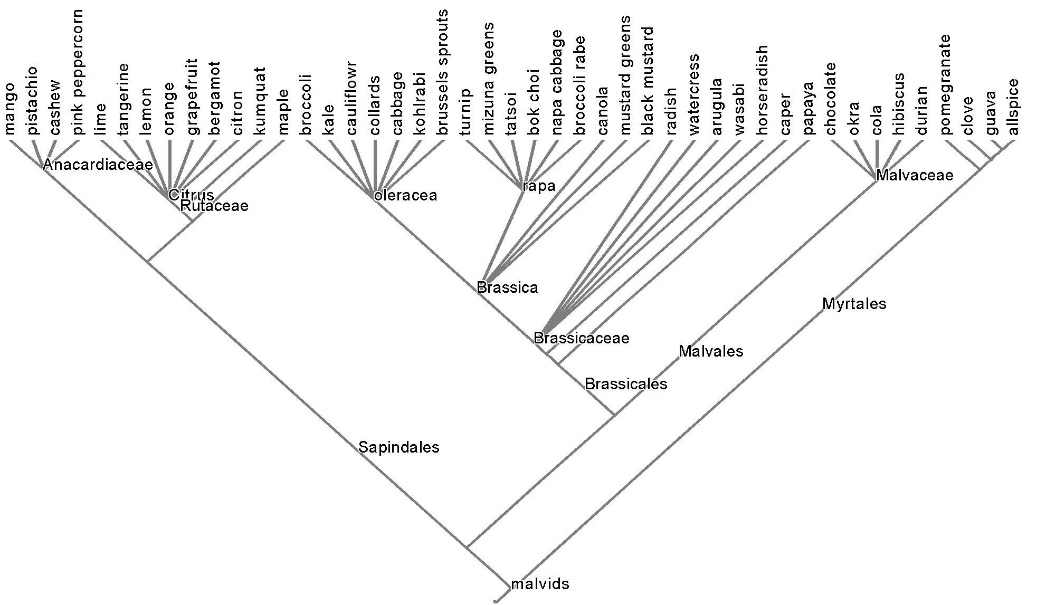
\includegraphics[height=3.82in]{./media/image3.jpeg}
	\end{center}\end{figure}


%%%%%%%%%%%%%%%%%%%% Figure/Image No: 3 Ends here %%%%%%%%%%%%%%%%%%%%

\vspace{\baselineskip}
Tree taxonomies are kinds of graphs that help you to better classify an object into several families of class and subclass. These kind of  taxonomy have oriented our research to choose our corporate taxonomy. \par

\begin{multicols}{2}

\vspace{\baselineskip}\vspace{\baselineskip}\vspace{\baselineskip}
A tree taxonomy is presented by this generic form \par

%%%%%%%%%%%%%%%%%%%% Figure/Image No: 4 starts here %%%%%%%%%%%%%%%%%%%%

\begin{figure}[H]
	\begin{center}		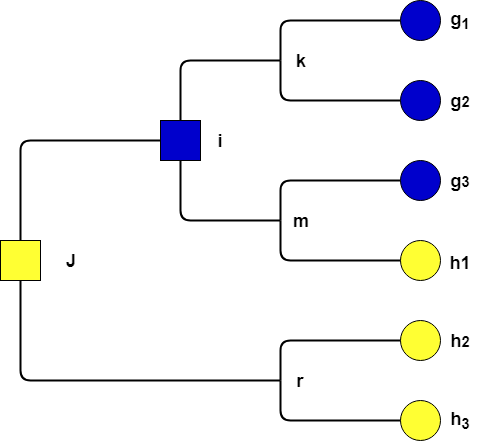
\includegraphics[width=2.82in,height=2.82in]{./media/image5.png}
	\end{center}\end{figure}


%%%%%%%%%%%%%%%%%%%% Figure/Image No: 4 Ends here %%%%%%%%%%%%%%%%%%%%
\end{multicols}

\newpage

\vspace{\baselineskip}\subsection*{The MISP  }
\addcontentsline{toc}{subsection}{The MISP  }

\vspace{\baselineskip}
The MISP’s team have of course create an engine to manage their taxonomies.  \par

Therefore, we have adapted our taxonomy to best fit their system\par


\vspace{\baselineskip}
\subsubsection*{Presentation}
\addcontentsline{toc}{subsubsection}{Presentation}

\vspace{\baselineskip}
The taxonomies of MISP are in the form:\par

\begin{Center}
{\fontsize{16pt}{19.2pt}\selectfont \textbf{ namespace.predicate = ``value’’}\par}
\end{Center}\par

\begin{itemize}
	\item Namespace\tab : Name of the taxonomy\par
	\item Predicate \tab : Object resource of the taxonomy\par
    \item •	Value\tab : Value of the resource\par
	\item  \tab :  resource  taxonom\par
\end{itemize}\par

As a result of these rules, we make the json in annexe 2 this annexe is here to describe how a generical taxonomy is written in order to be implemented directly in the MISP project.  \par

\subsubsection*{Main Advantages}
\addcontentsline{toc}{subsubsection}{Main Advantages}
Misp use taxonomies engine to create statistics, rate and classify events \par


\vspace{\baselineskip}
\subsubsection*{Main Drawbacks }
\addcontentsline{toc}{subsubsection}{Main Drawbacks }
\begin{itemize}
	\item	Without predicate parsing, the depth is limited to 1.\par

To avoid these drawback:\par

\begin{itemize}
	\item	A predicate could be parse to create multiple levels of tags and create a deeper taxonomy. Due to our need to depth, our parser will be the: \‘\’\_ \‘\’  \par

\begin{itemize}
	\item  Predicate: predicate = ‘’value’’  \par

\end{itemize}
\end{itemize}
	\item Long taxonomy can be problematic to use\par


\vspace{\baselineskip}
To avoid these drawback: \par

\begin{itemize}
	\item	A long taxonomy should have an interface for proper use\par

	\item	A complex need taxonomy need structuration to be used properly that why we will be inspired by other taxonomy in order to achieve that goal.
\end{itemize}
\end{itemize}\par

\newpage

\begin{multicols}{2}


\subsection*{Bugyuo Methodology}
\addcontentsline{toc}{subsection}{Bugyuo Methodology}

\vspace{\baselineskip}
\subsubsection*{Presentation}
\addcontentsline{toc}{subsubsection}{Presentation}
\begin{justify}
Security Methodology Project for Telecom Operators
\end{justify}\par

\begin{justify}
The infrastructure is generated by metrics that generate evidence that serves to minimize the risks that give a level of confidence on countermeasures that minimize risk.
\end{justify}\par

\begin{justify}
See the modification annexe to see the bugyo dendrogram use for this taxonomy.
\end{justify}\par

%%%%%%%%%%%%%%%%%%%% Figure/Image No: 3 starts here %%%%%%%%%%%%%%%%%%%%

\begin{figure}[H]	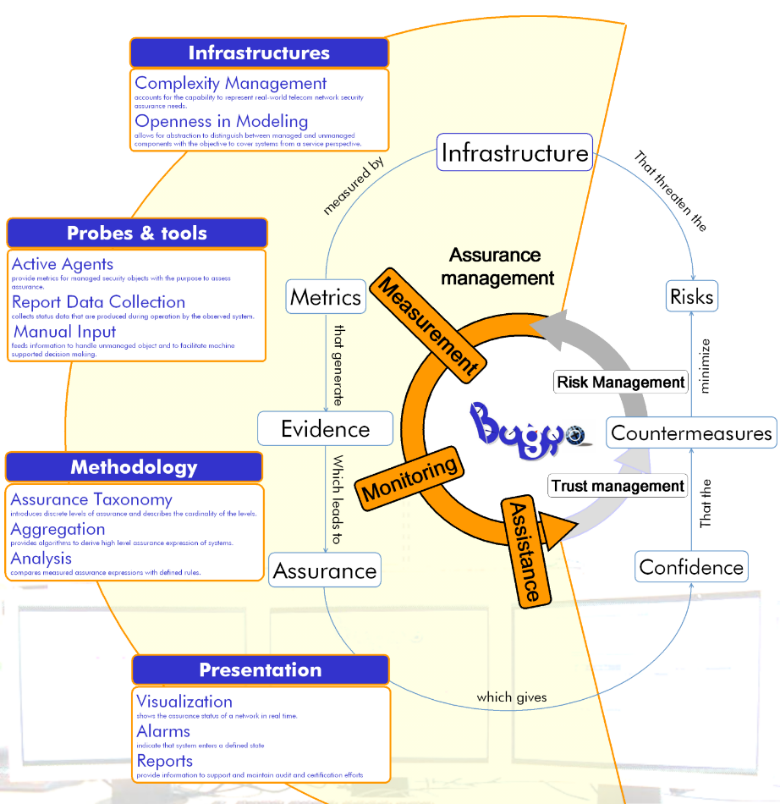
\includegraphics[width=3.54in,height=3.65in]{./media/image6.png}
\end{figure}


%%%%%%%%%%%%%%%%%%%% Figure/Image No: 3 Ends here %%%%%%%%%%%%%%%%%%%%


\end{multicols}

\subsubsection*{Main Advantages }
\addcontentsline{toc}{subsubsection}{Main Advantages }
\begin{itemize}
	\item Gives an interesting approach on the methodology of a security policy, security assurance and their different implementation and operation.
\end{itemize}\par

\begin{itemize}
	\item Gives an interesting approach on the methodology of a security policy, security assurance and their different implementation and operation. \par
	\item Created with the collaboration of one of our security teachers who come from Luxembourg.  \par
	\item Parallel approach to common criteria and deploys an interesting risks approach.
\end{itemize}\par

\subsubsection*{Main Drawbacks }
\addcontentsline{toc}{subsubsection}{Main Drawbacks }
\begin{itemize}
	\item Abstract concept which only give indications on how to proceed an engineer to securing a system\par
	\item The notions are very high in the methodological approach.\par
	\item Even though this representation is powerful, it is unknown to the general public
	
\end{itemize}\par

\subsubsection*{Conclusion }
\addcontentsline{toc}{subsubsection}{Conclusion }
\begin{justify}
To better understand the needs of an ISS, this methodology can help us to see if an event  responding to its needs.
These is a   these criteria have none really main methodology or program to applied them. 
In that goal, a methodology like bugyo could be  to check the advanced of these methodology in their enterprise. Many security events could be marked to follow the proper application of these stuff, furthermore a sharing  could be  to see how properly manage it.
The more the number of companies using it and sharing their ways of proceeding will increase,
the more it will be applied properly and understandable.
\end{justify}\par


 %%%%%%%%%%%%  Starting New Page here %%%%%%%%%%%%%%

\newpage

\subsection*{ ERCOT Faceted Classification  }
\addcontentsline{toc}{subsection}{ ERCOT Faceted Classification  }



%%%%%%%%%%%%%%%%%%%% Table No: 2 starts here %%%%%%%%%%%%%%%%%%%%


\begin{table}[H]
 			\centering
\begin{tabular}{p{0.71in}p{0.77in}p{0.7in}p{0.69in}p{0.66in}p{0.67in}p{0.69in}}
\hline
%row no:1
\multicolumn{1}{|p{0.71in}}{Function} & 
\multicolumn{1}{|p{0.77in}}{Activity} & 
\multicolumn{1}{|p{0.7in}}{Type} & 
\multicolumn{1}{|p{0.69in}}{Entity Type} & 
\multicolumn{1}{|p{0.66in}}{Entity} & 
\multicolumn{1}{|p{0.67in}}{Rule Type} & 
\multicolumn{1}{|p{0.69in}|}{System Name} \\
\hhline{-------}
%row no:2
\multicolumn{1}{|p{0.71in}}{Market: Participation} & 
\multicolumn{1}{|p{0.77in}}{Registration and Qualification} & 
\multicolumn{1}{|p{0.7in}}{Registration Documents} & 
\multicolumn{1}{|p{0.69in}}{Market Participant} & 
\multicolumn{1}{|p{0.66in}}{} & 
\multicolumn{1}{|p{0.67in}}{Protocol} & 
\multicolumn{1}{|p{0.69in}|}{} \\
\hhline{-------}
%row no:3
\multicolumn{1}{|p{0.71in}}{Information Technology} & 
\multicolumn{1}{|p{0.77in}}{System and Application Development} & 
\multicolumn{1}{|p{0.7in}}{Revision and Change Request} & 
\multicolumn{1}{|p{0.69in}}{Market Participant} & 
\multicolumn{1}{|p{0.66in}}{TDSP} & 
\multicolumn{1}{|p{0.67in}}{} & 
\multicolumn{1}{|p{0.69in}|}{MarkeTrak} \\
\hhline{-------}

\end{tabular}
 \end{table}


%%%%%%%%%%%%%%%%%%%% Table No: 2 ends here %%%%%%%%%%%%%%%%%%%%


\vspace{\baselineskip}


%%%%%%%%%%%%%%%%%%%% Table No: 3 starts here %%%%%%%%%%%%%%%%%%%%


\begin{table}[H]
 			\centering
\begin{tabular}{p{1.03in}p{1.03in}p{1.03in}}
\hline
%row no:1
\multicolumn{1}{|p{1.03in}}{\Centering Predicate } & 
\multicolumn{1}{|p{1.03in}}{\Centering	$\perp$ } & 
\multicolumn{1}{|p{1.03in}|}{\Centering Predicate } \\
\hhline{---}
%row no:2
\multicolumn{1}{|p{1.03in}}{\Centering Value  } & 
\multicolumn{1}{|p{1.03in}}{\Centering	$\perp$ } & 
\multicolumn{1}{|p{1.03in}|}{\Centering Value} \\
\hhline{---}
%row no:3
\multicolumn{1}{|p{1.03in}}{\Centering Value} & 
\multicolumn{1}{|p{1.03in}}{\Centering  $\perp$} & 
\multicolumn{1}{|p{1.03in}|}{\Centering Value} \\
\hhline{---}

\end{tabular}
 \end{table}


%%%%%%%%%%%%%%%%%%%% Table No: 3 ends here %%%%%%%%%%%%%%%%%%%%

Lexique : A $\perp$ B : A independent of B\par

Statically describes the operation of a business and its activities. \par

Each column describes a predicate of an instance from the service of the company for a proper purpose\par


\vspace{\baselineskip}
\subsubsection*{Main Advantages }
\addcontentsline{toc}{subsubsection}{Main Advantages }
\begin{itemize}
	\item Briefly presents the operation of a department of a company\par

	\item Hardcoded approach for corporate taxonomy \par

	\item	Representation which strongly resembling a multi-model-level (further details in this document)
\end{itemize}\par

\subsubsection*{Main Drawbacks }
\addcontentsline{toc}{subsubsection}{Main Drawbacks }
\begin{itemize}
	\item Too simple to use alone without another taxonomy\par
	\item All links of columns are independent from each other, it a drawback only if no other taxonomy is used to described how to fill the column\par

\end{itemize}\subsubsection*{ Conclusion}
\addcontentsline{toc}{subsubsection}{ Conclusion}
\begin{itemize}
	\item Despite these drawbacks these taxonomies could be used as a model for a properly structuration for another taxonomy like the one we decided to choose.  \par

	\item It could have inspired a way to present an object created with our taxonomy\par

As announced, the columns  is only a drawback if no other taxonomy is used, more over it became a strongly advantage in the goal of describe a multi-level-model.\par


 %%%%%%%%%%%%  Starting New Page here %%%%%%%%%%%%%%

\newpage

\vspace{\baselineskip}
\end{itemize}\subsection*{Architecting an Enterprise content management Strategy  }
\addcontentsline{toc}{subsection}{Architecting an Enterprise content management Strategy }

\vspace{\baselineskip}


%%%%%%%%%%%%%%%%%%%% Figure/Image No: 4 starts here %%%%%%%%%%%%%%%%%%%%

\begin{figure}[H]
	\begin{Center}
		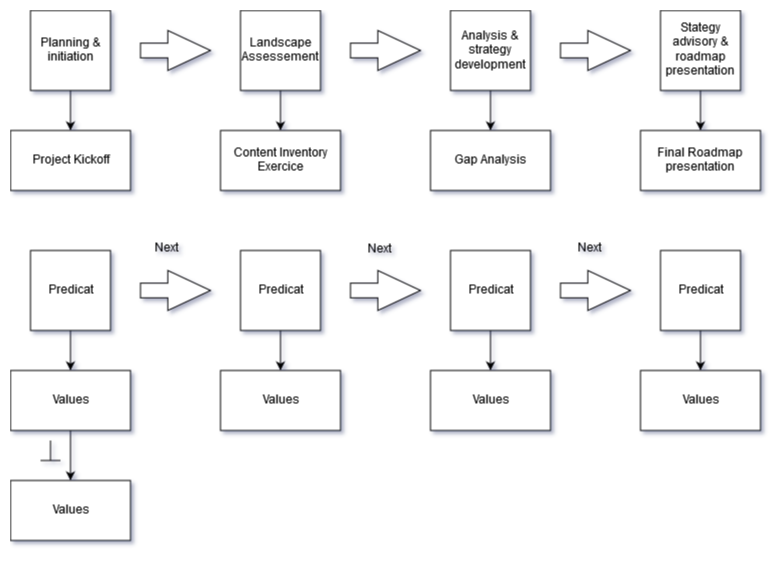
\includegraphics[width=6.3in,height=4.53in]{./media/image7.png}
	\end{Center}
\end{figure}


%%%%%%%%%%%%%%%%%%%% Figure/Image No: 4 Ends here %%%%%%%%%%%%%%%%%%%%

\par

Present the strategies of a company for the realization of a project. \par
The arrow presents the next instance that will be needed to realise the project.  \par
Each predicate could have many values, which will be independent between them. \par

\subsubsection*{Main Advantages }
\addcontentsline{toc}{subsubsection}{Main Advantages }
\begin{itemize}
	\item Present a taxonomy, in a timeline manner \par

	\item Could be useful to describe instance or event between them in a chronological manner\par


\end{itemize}\subsubsection*{Main Drawbacks }
\addcontentsline{toc}{subsubsection}{Main Drawbacks }
\begin{itemize}
	\item Does not in any way present the enterprise infrastructure, it’s useless for present jobs or objects  \par

\end{itemize}\subsubsection*{ Conclusion }
\addcontentsline{toc}{subsubsection}{ Conclusion }
\begin{itemize}
	\item Our job is not only to describe the infrastructure of an enterprise but all instance of an enterprise therefore it’s could be important to make some way to describe a chronological order for some plans of a company \par

	\item It could be an interesting way to structure a task in order to accomplish a company project.\par


 %%%%%%%%%%%%  Starting New Page here %%%%%%%%%%%%%%

\newpage

\vspace{\baselineskip}
\end{itemize}\subsection*{ Functional Classification Taxonomies }
\addcontentsline{toc}{subsection}{ Functional Classification Taxonomies}


%%%%%%%%%%%%%%%%%%%% Figure/Image No: 5 starts here %%%%%%%%%%%%%%%%%%%%

\begin{figure}[H]
	\begin{Center}
		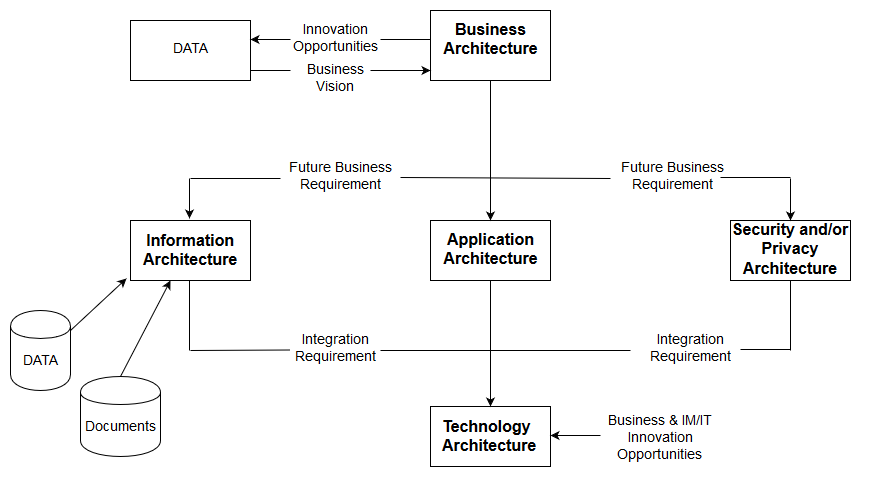
\includegraphics[width=6.56in,height=3.04in]{./media/image8.png}
	\end{Center}
\end{figure}


%%%%%%%%%%%%%%%%%%%% Figure/Image No: 5 Ends here %%%%%%%%%%%%%%%%%%%%

This graphics explain how for them a data is share in some architecture:   \par

\begin{itemize}
	\item Business: harvest the data information\par

	\item Information: store the data in some disks\par

	\item Application: Use this data for the purpose of the company \par

	\item Security / privacy  Secure the data harvested\par

	\item Technology: has been used by the application part to process the data \par
\end{itemize}\par



%%%%%%%%%%%%%%%%%%%% Figure/Image No: 6 starts here %%%%%%%%%%%%%%%%%%%%

\begin{figure}[H]
	\begin{Center}
		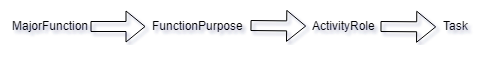
\includegraphics[width=5.25in,height=0.67in]{./media/image9.png}
	\end{Center}
\end{figure}


%%%%%%%%%%%%%%%%%%%% Figure/Image No: 6 Ends here %%%%%%%%%%%%%%%%%%%%

\begin{Center}
Business / Application / Technical / Information


Define links between the major instances of an archetype company. \par

 Education \textbf{=>} Teach \textbf{=>} Teacher \textbf{=> }Network course \par
\end{Center}

\subsubsection*{Main Advantages }
\addcontentsline{toc}{subsubsection}{Main Advantages }
\begin{itemize}
	\item The major instances of a company could be linked thanks to that \par
\end{itemize}
\subsubsection*{Main Drawbacks }
\addcontentsline{toc}{subsubsection}{Main Drawbacks }
\begin{itemize}
	\item Doesn’t explain what is an instance of an enterprise  \par


\end{itemize}\subsubsection*{Conclusion }
\addcontentsline{toc}{subsubsection}{ Conclusion }
\begin{itemize}
	\item The main idea of linking could be used to linked other instances from a taxonomy more complex like the GEA-NZ taxonomy \par



 %%%%%%%%%%%%  Starting New Page here %%%%%%%%%%%%%%

\newpage

\vspace{\baselineskip}
\end{itemize}\subsection*{Sector Taxonomy and definitions}
\addcontentsline{toc}{subsection}{Sector Taxonomy and definitions}

\vspace{\baselineskip}


%%%%%%%%%%%%%%%%%%%% Figure/Image No: 7 starts here %%%%%%%%%%%%%%%%%%%%

\begin{figure}[H]
	\begin{Center}
		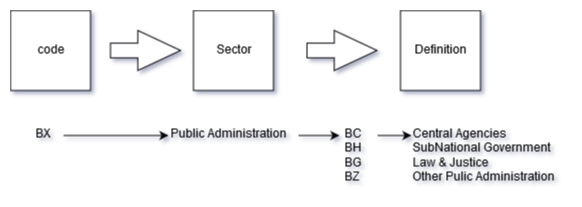
\includegraphics[width=6.06in,height=2.16in]{./media/image10.png}
	\end{Center}
\end{figure}


%%%%%%%%%%%%%%%%%%%% Figure/Image No: 7 Ends here %%%%%%%%%%%%%%%%%%%%

 \par

\begin{Center}
Interesting mapping of instances of jobs from any sector of activity
\end{Center}\par

\subsubsection*{Main Advantages }
\addcontentsline{toc}{subsubsection}{Main Advantages }
\begin{itemize}
	\item Professional directory of classification\par

	\item Easy way to research an instance once the code is know\par


\end{itemize}\subsubsection*{Main Drawbacks }
\addcontentsline{toc}{subsubsection}{Main Drawbacks }
\begin{itemize}
	\item More a directory of job than a real taxonomy \par


\end{itemize}\subsubsection*{ Conclusion }
\addcontentsline{toc}{subsubsection}{ Conclusion }
\begin{itemize}
	\item It could be interesting, once our taxonomy operational to map our instance realised thanks to that way and a hierarchical methods\par


\vspace{\baselineskip}

\vspace{\baselineskip}

\end{itemize}\subsection*{Taxonomy code mapping / professional providers }
\addcontentsline{toc}{subsection}{Taxonomy code mapping / professional providers }

\vspace{\baselineskip}
It’s a directory of instance, consequently it’s presented the exact same advantages and drawbacks than the previous Sector Taxonomy and definitions.\par


\vspace{\baselineskip}

\vspace{\baselineskip}


 %%%%%%%%%%%%  Starting New Page here %%%%%%%%%%%%%%

\newpage

\vspace{\baselineskip}\subsection*{ICB Version 2: IPMA Competence Baseline}
\addcontentsline{toc}{subsection}{ICB Version 2: IPMA Competence Baseline}
Example of ICB-Version  page 74 \par



%%%%%%%%%%%%%%%%%%%% Figure/Image No: 8 starts here %%%%%%%%%%%%%%%%%%%%

\begin{figure}[H]
	\begin{Center}
		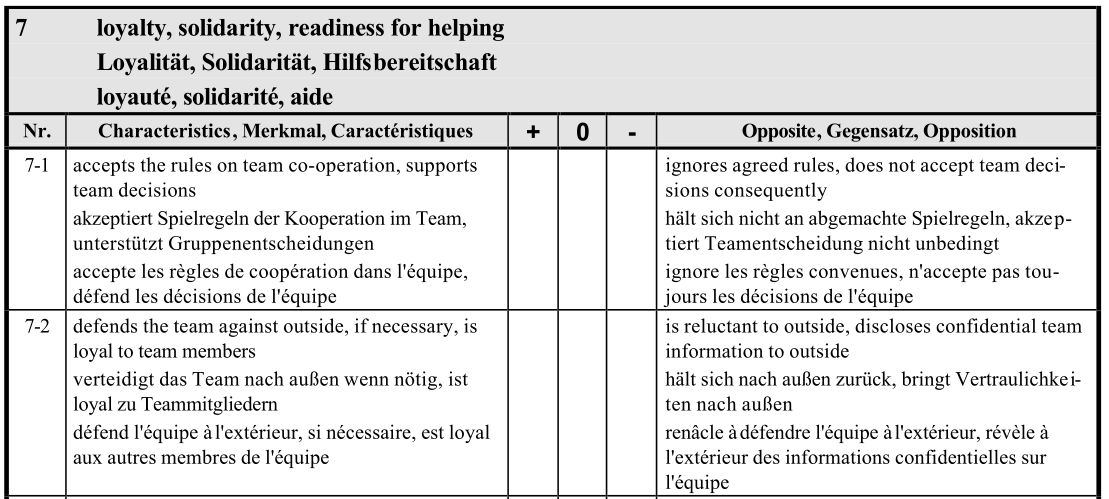
\includegraphics[width=6.3in,height=2.83in]{./media/image11.png}
	\end{Center}
\end{figure}


%%%%%%%%%%%%%%%%%%%% Figure/Image No: 8 Ends here %%%%%%%%%%%%%%%%%%%%

\par

A taxonomy asking a company of their competence.  \par

Present a really interesting way to make a survey in order to create an instance from this taxonomy.\par


\vspace{\baselineskip}
\subsubsection*{Main Advantages }
\addcontentsline{toc}{subsubsection}{Main Advantages }
\begin{itemize}
	\item The survey is a really interesting and easy way to asking a thing to a customer\par

\vspace{\baselineskip}
\end{itemize}\subsubsection*{Main Drawbacks }
\addcontentsline{toc}{subsubsection}{Main Drawbacks }
\begin{itemize}
	\item The taxonomy itself isn’t really interesting to make a corporate taxonomy\par

\vspace{\baselineskip}
\end{itemize}\subsubsection*{ Conclusion }
\addcontentsline{toc}{subsubsection}{ Conclusion }
\begin{itemize}
	\item Once our taxonomy is designed we could use this way to ask for create dynamically some instance of our taxonomy.\par



 %%%%%%%%%%%%  Starting New Page here %%%%%%%%%%%%%%

\newpage

\vspace{\baselineskip}
\end{itemize}\subsection*{GEA-NZ: Government Enterprise Architecture New-Zealand }
\addcontentsline{toc}{subsection}{GEA-NZ: Government Enterprise Architecture New-Zealand }


%%%%%%%%%%%%%%%%%%%% Figure/Image No: 9 starts here %%%%%%%%%%%%%%%%%%%%

\begin{figure}[H]
	\begin{Center}
		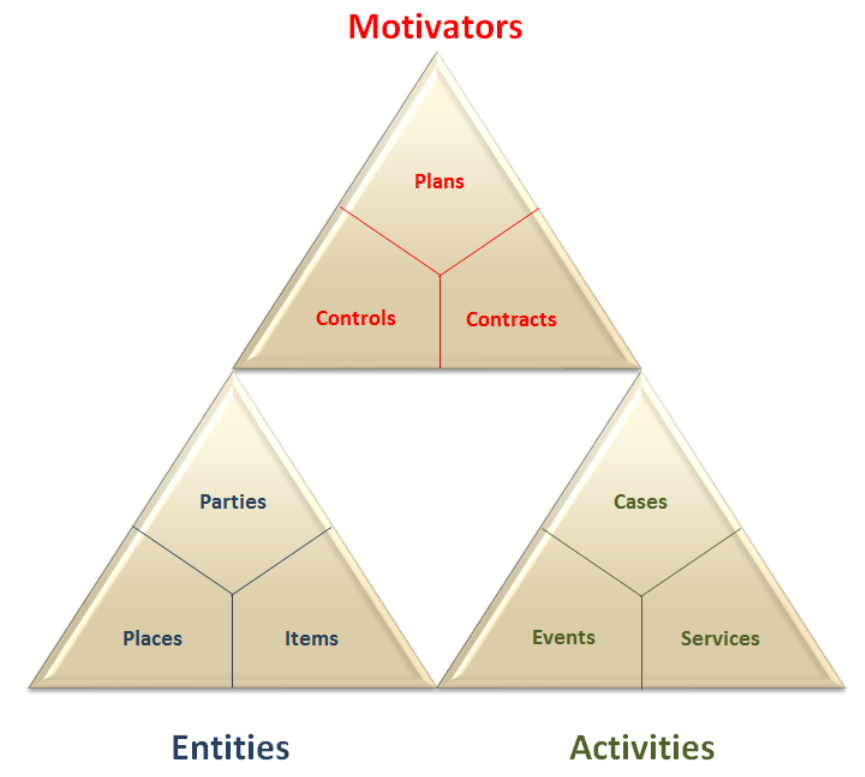
\includegraphics[width=3.29in,height=2.96in]{./media/image12.png}
	\end{Center}
\end{figure}


%%%%%%%%%%%%%%%%%%%% Figure/Image No: 9 Ends here %%%%%%%%%%%%%%%%%%%%

\par

The taxonomy that has been choose by us.\par

Thanks to three complete tables also divided in three branches \\
Note : 	See the annexe 2 to see the main branch presented without their leaf for more readability
See the NGA-NZ for properly instructions about their leaf, the taxonomy being used as it is been , the rewrite here would have no interest except for the add we made of it.\par

\subsubsection*{Description of the main branch}
\addcontentsline{toc}{subsubsection}{Description of the main branch}
\begin{itemize}
	\item \textbf{Motivator: } Purpose \par

\begin{itemize}
	\item \textbf{ Plans:}actions accomplished for choose a direction\par
	\item \textbf{Controls:}the constraints of actions\par
	\item \textbf{Contracts: }agreement between different parties\par

\end{itemize}
	\item \textbf{Entities: }all possibly instances in  enterprise \par

\begin{itemize}
	\item \textbf{Places:}Workplace and any location\par

	\item \textbf{Items:}All items buyable or not\par

	\item \textbf{Parties:}Staff entities\par


\end{itemize}
	\item \textbf{Activities:}all possibly interaction between parties\par

\begin{itemize}
	\item \textbf{Cases:}Special and normal event managed\par

	\item \textbf{Events:}Planning and / or Spontaneous event\par

	\item \textbf{Services:}Offer of the service\par


\end{itemize}
\end{itemize}
\newpage
\subsubsection*{Main Advantages }
\addcontentsline{toc}{subsubsection}{Main Advantages }
\begin{itemize}
	\item A really complete cooperative taxonomy for each instances of an enterprise\par

\end{itemize}

\subsubsection*{Main Drawbacks }
\addcontentsline{toc}{subsubsection}{Main Drawbacks }
\begin{itemize}
	\item It’s as complete as it is complex to use, that’s why It’s need a structuration for a properly usage\par
	\item Some names could be put in a generic: new-zealand could be replaced by enterprise headquarter \par


\end{itemize}\subsubsection*{ Conclusion }
\addcontentsline{toc}{subsubsection}{Conclusion }

This taxonomy is powerful but it does not force any structuring to make some object like : jobs, activities. \par \par
This structure is crucial to make some classification furthermore.




 %%%%%%%%%%%%  Starting New Page here %%%%%%%%%%%%%%

\newpage

\vspace{\baselineskip}\section*{Modification of GEA-NZ }
\addcontentsline{toc}{section}{Modification of GEA-NZ }
Note: Please see the Annexe 3 for the picture of adaptation into GEA-NZ taxonomy. \par
In purpose to make the control region more accurate we add two more sub-category. \par

\subsection*{Risk Governance}
\addcontentsline{toc}{subsection}{Risk Governance}
\begin{itemize}
	\item Risk Governance in order to evaluate the risk taken with the object\par

\begin{itemize}
	\item \textbf{Residual Risk : }This element is a remaining risk in the enterprise\par

	\item \textbf{Risk Analysis :} Risk  by the enterprise\par

	\item \textbf{Risk Assessment : } General process of analysis and risk assessment \par

	\item \textbf{Risk Management :  } Control and organize the activity taking into account the risks \par

	\item \textbf{Risk Treatment : } Measures selections and implements the chosen metrics
\end{itemize}\par


\end{itemize}\subsection*{Bugyo }
\addcontentsline{toc}{subsection}{Bugyo }
\begin{itemize}
	\item Bugyo in order to add some security methodology in the code to verify directly a component\par
\end{itemize}

\begin{itemize}
	\item \textbf{Service model:} applied to the model as a whole\par

\begin{itemize}
	\item \textbf{ Absence of relevant vulnerability   }\par

\begin{itemize}
	\item Is a vulnerability present? yes // no?\par


\end{itemize}
	\item \textbf{Unmanaged/Managed Ratio}\par

\begin{itemize}
	\item Less Unmanaged / Higher confidence about the ratio ? \par
\end{itemize}
\end{itemize}
	\item \textbf{Maintenance Management } applied to the model to see the maintenance of it \par

\begin{itemize}
	\item \textbf{Probe Maintenance:} Is the maintenance \par

\begin{itemize}
	\item \textbf{Reactive :}  Ad-hoc maintenance / maintenance policy  present ? \par

	\item \textbf{Pro-active:} Regular interval to prevent / Documentation and log \par


\end{itemize}
	\item  \textbf{Infrastructure object model maintenance: } maintenance for each object  \par

\begin{itemize}
	\item \textbf{Reactive :}  Ad-hoc maintenance / maintenance policy present?   \par

	\item \textbf{Pro-active:}  Regular interval to prevent / Documentation and log\par


\end{itemize}
\end{itemize}
\newpage
	\item \textbf{Metric Construction:  } is used to measure the system's security policy \par

\begin{itemize}
	\item \textbf{Scope:}request the number of elements measured by the system \par

\begin{itemize}
	\item Are there countermeasure? How much it’s goes around the system?  \par

\end{itemize}

	\item \textbf{Depth: } How for in details it’s goes?  \par

\begin{itemize}
	\item Is there an interface for?  \par

\begin{itemize}
	\item o	A single object? The whole chain?   \\
The whole chain and all the values passing through it.\par


\end{itemize}
\end{itemize}
	\item \textbf{Rigor:  }How is the formalism of the measures? Is it strict?  \par

\begin{itemize}
	\item None verification / informal-verification / semiformal verification    \par


\end{itemize}
	\item \textbf{ Reliability of metric }Are the measure repeatable?  \par

\begin{itemize}
	\item	None verification / reproductible / informally / semiformal \par


\end{itemize}
	\item \textbf{ Timeliness:  }How recent are the software? \par

\begin{itemize}
	\item None verification / Version prior the newest (if retro compatible)  \\
Most recent version (Avoiding flaws with patch)  \par


\end{itemize}
	\item \textbf{Frequency: } How fresh is the evidence of measure? \par

\begin{itemize}
	\item \textbf{ }Year / Month / Week / Day / Hours\par


\end{itemize}
	\item \textbf{Stability:  }How stable is the measure \par

\begin{itemize}
	\item Is there a human avoiding False/True positive? \\ Or / And are there statistics algorithms? \par


\end{itemize}
\end{itemize}
\end{itemize}

\newpage

\section*{The multi-level-model (MLM) }
\addcontentsline{toc}{section}{The multi-level-model (MLM) }
Multilevel models (also known as hierarchical linear models, nested data models, mixed models, random coefficient, random-effects models, random parameter models, or split-plot designs) are statistical models of parameters that vary at more than one level.  \par

 A multi-level-model is created when a complex structuration is used and require different cutting levels.    \par

Each region could have many states and each state could have many observations and so on.\par



%%%%%%%%%%%%%%%%%%%% Figure/Image No: 10 starts here %%%%%%%%%%%%%%%%%%%%


\begin{figure}[H]	\begin{subfigure}		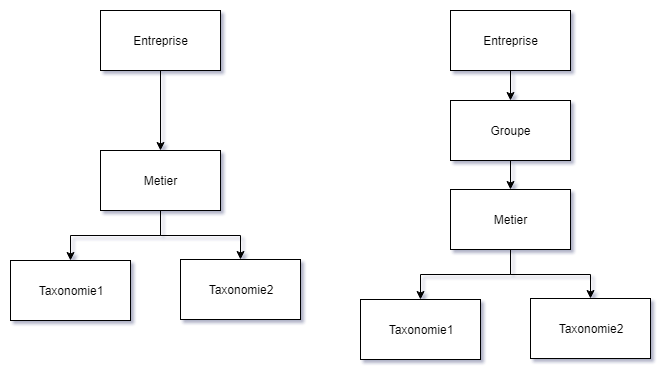
\includegraphics[width=0.45\textwidth]{./media/image13.png}
	\end{subfigure}
~	\begin{subfigure}		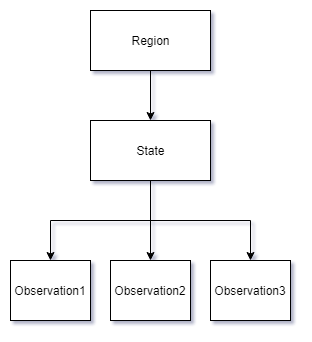
\includegraphics[width=0.45\textwidth]{./media/image14.png}
	\end{subfigure}
~
\end{figure}


%%%%%%%%%%%%%%%%%%%% Figure/Image No: 10 Ends here %%%%%%%%%%%%%%%%%%%%


\vspace{\baselineskip}
\textbf{\textit{Generical Taxonomy  \tab enterprise job\tab enterprise service of job }}\par

\vspace{\baselineskip}

\begin{multicols}{2}

%%%%%%%%%%%%%%%%%%%% Figure/Image No: 11 starts here %%%%%%%%%%%%%%%%%%%%

\begin{figure}[H]
	\begin{Center}
		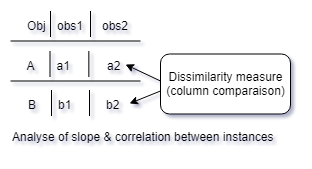
\includegraphics[width=234.15pt,height=126.9pt]{./media/image15.png}
	\end{Center}
\end{figure}



%%%%%%%%%%%%%%%%%%%% Figure/Image No: 11 Ends here %%%%%%%%%%%%%%%%%%%%

For each object created we have a level and for of the  could be used\par\par

In order to make possible this stuff we could make for each type of object a table in order to compare an object between another object of the same type. (like job, service)\par

Once a table is made for an object, we can observe a dissimilarity measure, reporting differences between the different columns.\par

\end{multicols}
\begin{multicols}{2}

%%%%%%%%%%%%%%%%%%%% Figure/Image No: 16 starts here %%%%%%%%%%%%%%%%%%%%

\begin{figure}[H]
	\begin{Center}
		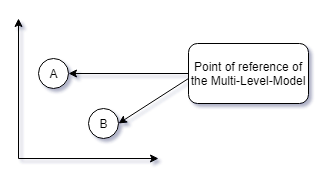
\includegraphics[width=247.6pt,height=141.95pt]{./media/image16.png}
	\end{Center}
\end{figure}


%%%%%%%%%%%%%%%%%%%% Figure/Image No: 16 Ends here %%%%%%%%%%%%%%%%%%%%

In the end, we can make a graphics thanks to the dissimilarity measure to make a graphics of point of reference for each object. \par
As a result, with these graphics we can make an HAC (Hierarchical Ascending Classification

\end{multicols}

 %%%%%%%%%%%%  Starting New Page here %%%%%%%%%%%%%%

\newpage

\vspace{\baselineskip}\section*{Hierarchical Ascending Classification (HAC)}
\addcontentsline{toc}{section}{Hierarchical Ascending Classification (HAC)}
In data mining and statistics, hierarchical clustering (also called hierarchical cluster analysis or HCA) is a method of cluster analysis which seeks to build a hierarchy of clusters. \par

An HAC is created  \par

\begin{itemize}
	\item a  is needed\par

	\item \textbf{dissimilarity  measure }\par

	\item for clustering many  in order to make cluster analysis and segmentation.
\end{itemize}\par

\textbf{Once created, this cluster will make it possible to present wiser choices to the client.}\par

Point  \par

\begin{itemize}
	\item As see  each point will present an object created with the taxonomy 
\end{itemize}\par

Strategies for hierarchical clustering generally fall into two \par

\begin{itemize}
	\item \textbf{Agglomerative:} This is a "\textbf{bottom-up}" approach: each observation starts in its own cluster, and pairs of clusters are merged as one moves up the hierarchy.\par

	\item \textbf{Divisive:} This is a "\textbf{top-down}" approach: all observations start in one cluster, and splits are performed recursively as one moves down the hierarchy.
\end{itemize}\par

\begin{multicols}{2}

%%%%%%%%%%%%%%%%%%%% Figure/Image No: 13 starts here %%%%%%%%%%%%%%%%%%%%

\begin{figure}[H]
\advance\leftskip -0.18in		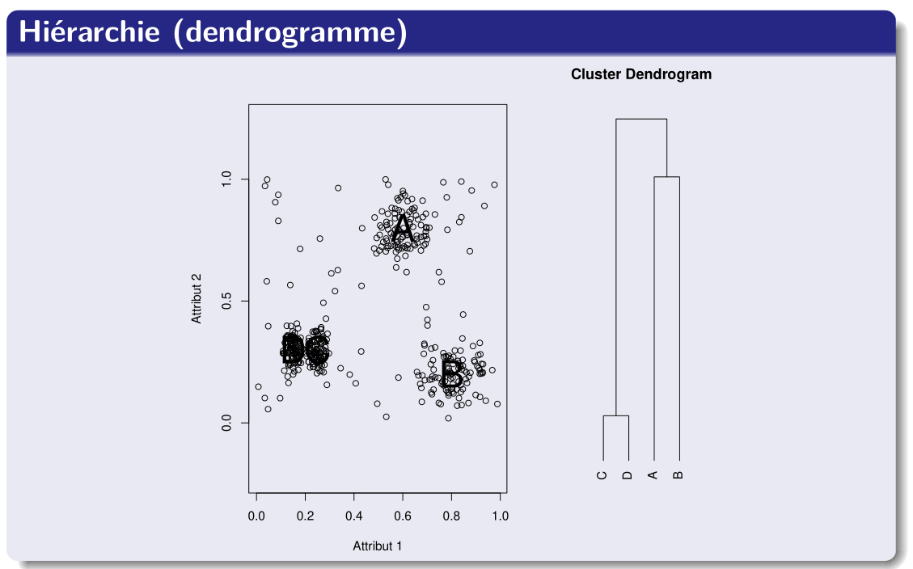
\includegraphics[width=3.15in,height=1.59in]{./media/image17.png}
\end{figure}


%%%%%%%%%%%%%%%%%%%% Figure/Image No: 13 Ends here %%%%%%%%%%%%%%%%%%%%
These algorithms are usually based on distance (prototype or density) and / or Grid-based like Dendrogram (discretization of data) \par
These methods can make their own concept thanks to cloud of points \par
The cluster dendogram will be the final goal of this project \par

\end{multicols}

\begin{multicols}{2}


%%%%%%%%%%%%%%%%%%%% Figure/Image No: 14 starts here %%%%%%%%%%%%%%%%%%%%

\begin{figure}[H]
\advance\leftskip -0.36in		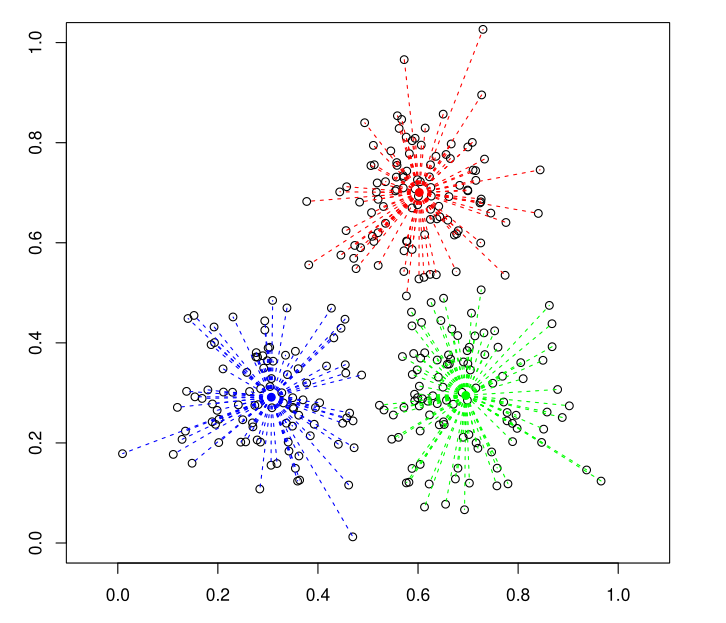
\includegraphics[width=3.16in,height=2.71in]{./media/image18.png}
\end{figure}


%%%%%%%%%%%%%%%%%%%% Figure/Image No: 14 Ends here %%%%%%%%%%%%%%%%%%%%
This picture represent a method based on prototypes
\begin{itemize}
\item A prototype is:
\begin{itemize}
  \item A representative individual 
  \item A seed (called an Isobarycenter*)
\end{itemize}\end{itemize}
The center of each class is also called an isobarycenter
\par Finally, once this step arrived we must minimised by calculating the intra class inertia and then deducing each class for each object and their relation among them in order to finally made the final cluster dendrogram.


\end{multicols}

%%%%%%%%%%%%%%%%%%%% new page %%%%%%%%%%%%%%%%%%%%
\newpage

\vspace{\baselineskip}\section*{Algorithms K-MEANS}
\addcontentsline{toc}{section}{Algorithms K-MEANS}

The K-means method is an optimization algorithm of intra-class inertia \par

\subsubsection*{Algorithms Names}
\addcontentsline{toc}{subsubsection}{Algorithms Names}
\begin{itemize}
\item K-means, K-moyennes, K-noyaux
\item Algorithm of dynamic clouds, mobile centers
\item Lloyd’s algorithm
\end{itemize}

\subsubsection*{The algorithm K-MEANS to determine new class and there Isobarycenter}
\addcontentsline{toc}{subsubsection}{The algorithm K-MEANS to determine new class and there Isobarycenter}

\subsubsection*{Description}
\addcontentsline{toc}{subsubsection}{Description}

\begin{itemize}
\item Alternation of two stages:

\begin{itemize}
\item Grouping objects into classes around centers
\item Adjustment of centers according to the component objects classes
\end{itemize}

\item Stopping the algorithm when there is no more change (or after a fixed number of iterations)
\item Convergence of the algorithm in a guaranteed finite time //
(usually correct result in 10 iterations)

\end{itemize}


\subsubsection*{Realization}
\addcontentsline{toc}{subsubsection}{Realization}
\begin{itemize}
\item Random initialization of centers
\item As long as the result varies
\end{itemize}
\begin{itemize}
\item For all objects
\begin{itemize}
\item Calculate the distance to all centers
\item Assign the object to the class most close
\end{itemize}
\item For all classes
\begin{itemize}
\item Calculate the center of gravity of the objects assigned
\item Assign the center of gravity as new center of the class
\end{itemize}
\end{itemize}

\vspace{\baselineskip}

The K-means methods will only serve to create each class, the final cluster dendrogram will be created thanks to the UPGMA methods for more precision see the annexe document to made the clustering.

\newpage

\section*{UPGMA : pair group method with arithmetic mean}
\addcontentsline{toc}{section}{UPGMA : pair group method with arithmetic mean}

The UPGMA algorithm constructs a rooted tree (dendrogram) that reflects the structure present in a pairwise similarity matrix (or a dissimilarity matrix). At each step, the nearest two clusters are combined into a higher-level cluster. 
The distance between any two clusters A and B each of size.

\subsubsection*{Determine the matrix for UPGMA}
\addcontentsline{toc}{subsubsection}{Determine the matrix for UPGMA}

\begin{itemize}
\item initialize the matrix A
\begin{itemize}
\item For all objects classes
\end{itemize}
\begin{itemize}
\item Calculate the distance to all others objects class
\end{itemize}
\item Make the UPGMA algorithm
\end{itemize}

\subsubsection*{Algorithm}
\addcontentsline{toc}{subsubsection}{Algorithm}

The UPGMA algorithm constructs a rooted tree (dendrogram) that reflects the structure present in a pairwise similarity matrix (or a dissimilarity matrix). At each step, the nearest two clusters are combined into a higher-level cluster. The distance between any two clusters A and B , each of size (i.e., cardinality) |A | and |B|,is taken to be the average of all distance d(x,y) between pairs of objects x in A and y in B, that is, the mean distance between elements of each cluster:
 
 
\begin{figure}[H]
	\begin{center}		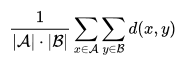
\includegraphics[width=2.8in,height=1.0in]{./media/image19.png}
	\end{center}\end{figure}
 
 
In other words, at each clustering step, the updated distance between the joined clusters A U B and and a new cluster X is given by the proportional averaging of the dA,X and dB,X distances:
 
 
\begin{figure}[H]
	\begin{center}		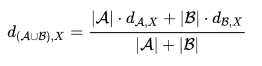
\includegraphics[width=3.3in,height=1.0in]{./media/image20.png}
	\end{center}\end{figure}
 
The UPGMA algorithm produces rooted dendrograms and requires a constant-rate assumption - that is, it assumes an ultrametric tree in which the distances from the root to every branch tip are equal. When the tips are molecular data (i.e., DNA, RNA and protein), the ultrametricity assumption is called the molecular clock.

\newpage

\section*{Create an Object with GEA-NZ}
\addcontentsline{toc}{section}{Create an Object with GEA-NZ }

GEA-NZ with the change made in annexe will be use see the taxonomy itself for have the leaf of the taxonomy. To adapted to MISP the GEA-NZ will be transform into MISP J-SON see the documents GEA-json for implementation.

\begin{itemize}
\item All new object will be added dynamically to the directory and class object in consequence of applying the methodology explained below
\end{itemize}



\subsubsection*{How It Will Works?}
\addcontentsline{toc}{subsubsection}{How It Will Works?}

\begin{itemize}
\item For each type of object wanted like Job, Activities, Items
    \begin{itemize}
    \item A table will be made and use as a template to made a Multi-level-model representation which each tables will have independency between columns
        \begin{itemize}
        \item For structural instances, we can make a table on the the ERCOT Faceted Classification example
        \item For type of activities, we can make a table on the “Architecting an Enterprise content management Strategy” example 
        \end{itemize}
    \end{itemize}
    \item Each column of the table template will be fill with the GEA-NZ 
    \item Once each columns are filled, a dissimilatory measure can be made
    \item Thanks to the dissimilatory measure, we can fill a graphics with points of object instance 
    \item Each points could be regrouping with the K-means method, it will make our object class
    \item A matrix grouping all the object class with each distance among them is made
    \item Thanks to the matrix, once created, we can apply the UPGMA method in order to create the clustering dendrogram.
    \item Now complete directory grouping all the instance object and their class could be made to simplify the creation of further users.

\end{itemize}


\subsubsection*{Applied It on MISP ?}
\addcontentsline{toc}{subsubsection}{ Applied It on MISP ?}

\begin{itemize}
\item Thanks to the clustering dendrogram and the directory a user could made and choose a job created or modify an existent object.
\item To simplify the creation of user, an alternate survey could be made as the ICB Version 2: IPMA Competence Baseline methods 
\item MISP present many different events, for each representative event, we will must make a template object for each particular type in order to represent it with this methodology.

\begin{itemize}
    \item	Bugyo and risk governance are added to apply a security approach to the taxonomy 
\end{itemize}
\end{itemize}


\newpage
%%%%%%%%%%%%%%%%%%%% new page %%%%%%%%%%%%%%%%%%%%
\vspace{\baselineskip}\section*{Annexe 2 : GEA-NZ : Government Entprise Architecture New -Zealand}
\addcontentsline{toc}{section}{Annexe 2 : GEA-NZ : Government Entprise Architecture New -Zealand}


%%%%%%%%%%%%%%%%%%%% Figure/Image No: 15 starts here %%%%%%%%%%%%%%%%%%%%

\begin{figure}[H]
	\begin{center}		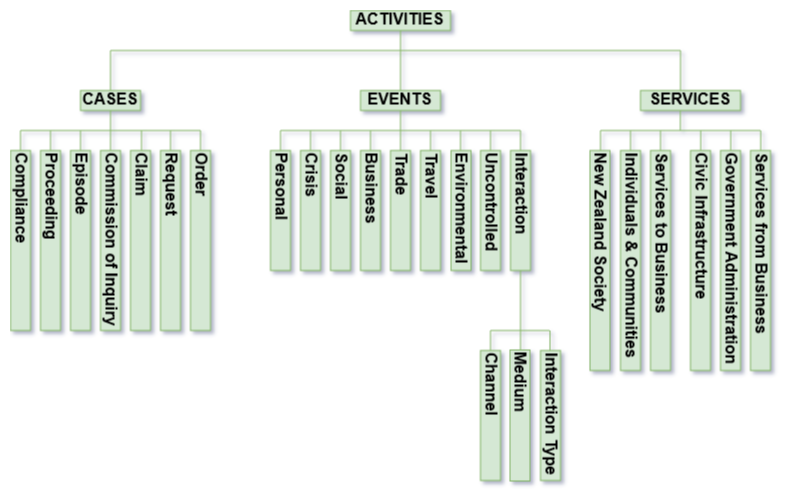
\includegraphics[width=5.3in,height=3.0in]{./media/image21.png}
	\end{center}\end{figure}


%%%%%%%%%%%%%%%%%%%% Figure/Image No: 15 Ends here %%%%%%%%%%%%%%%%%%%%



%%%%%%%%%%%%%%%%%%%% Figure/Image No: 16 starts here %%%%%%%%%%%%%%%%%%%%

	\begin{center}
\begin{figure}[H]	\begin{subfigure}		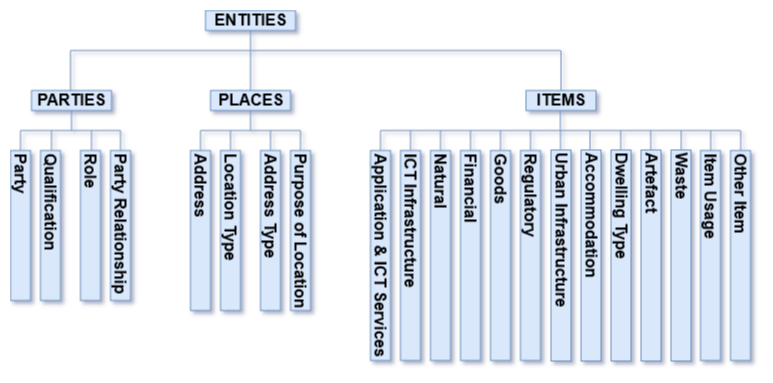
\includegraphics[width=0.75\textwidth]{./media/image22.png}
	\end{subfigure}
	\vspace{\baselineskip}
	\vspace{\baselineskip}
\vspace{\baselineskip}
\vspace{\baselineskip}

~	\begin{subfigure}		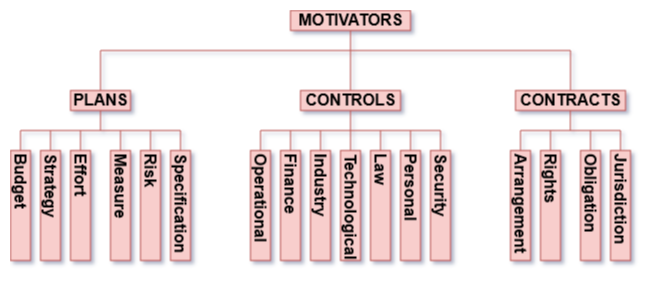
\includegraphics[width=0.75\textwidth]{./media/image23.png}
	\end{subfigure}
~
\end{figure}
\end{center}

%%%%%%%%%%%%%%%%%%%% Figure/Image No: 16 Ends here %%%%%%%%%%%%%%%%%%%%



 %%%%%%%%%%%%  Starting New Page here %%%%%%%%%%%%%%

\newpage
\par

\section*{Annexe 2 : Generical Taxinomy JSON}
\addcontentsline{toc}{section}{Annexe 2 : Generical Taxinomy JSON}
\setlength{\parskip}{0.0pt}
$ \{ $ \  namespace": "Title of your Taxonomy",\par

\  "description": "Taxonomy to classify the information of ... .",\par

\  "refs": [\par

\ \ \  "url ... "\par

\  ],\par

\  "version": 1,\par

\  "predicates": [\par

\ \ \  $ \{ $ \par

\ \ \ \ \  "value": "Name1 ",\par

\ \ \ \ \  "expanded": "Expanded Name 1 ",\par

\ \ \ \ \  "description": "TDesciption of the name 1"\par

\ \ \  $ \} $ ,\par

\ \ \  $ \{ $ \par

\ \ \ \ \  "value": "Name2 ",\par

\ \ \ \ \  "expanded": "Expanded Name 2 ",\par

\ \ \ \ \  "description": "TDesciption of the name 2"\par

\ \ \  $ \} $ \par

\  ],\par

\  "values": [\par

\ \ \  $ \{ $ \par

\ \ \ \ \  "predicate": "Name1",\par

\ \ \ \ \  "entry": [\par

\ \ \ \ \ \ \  $ \{ $ \par

\ \ \ \ \ \ \ \ \  "value": " value1 ",\par

\ \ \ \ \ \ \ \ \  "expanded": "Def Value1"\par

\ \ \ \ \ \ \  $ \} $ ,\par

\ \ \ \ \ \ \  $ \{ $ \par

\ \ \ \ \ \ \ \ \  "value": "value2",\par

\ \ \ \ \ \ \ \ \  "expanded": "Def Value2"\par

\ \ \ \ \ \ \  $ \} $ \par

\ \ \ \ \  ]\par

\ \ \  $ \} $ ,\par

\ \ \  $ \{ $ \par

\ \ \ \ \  "predicate": "Name2",\par

\ \ \ \ \  "entry": [\par

\ \ \ \ \ \ \  $ \{ $ \par

\ \ \ \ \ \ \ \ \  "value": " value1 ",\par

\ \ \ \ \ \ \ \ \  "expanded": "Def Value1"\par

\ \ \ \ \ \ \  $ \} $ ,\par

\ \ \ \ \ \ \  $ \{ $ \par

\ \ \ \ \ \ \ \ \  "value": "value2",\par

\ \ \ \ \ \ \ \ \  "expanded": "Def Value2"\par

\ \ \ \ \ \ \  $ \} $ \par

\ \ \ \ \  ]\par

\ \ \  $ \} $ \par

\  ]$ \} $ \par

\setlength{\parskip}{8.04pt}
\section*{Annexe 3 : Modification of GEA-NZ}
\addcontentsline{toc}{section}{Annexe 3 : Modification of GEA-NZ}
Bugyo and a risk gouvernance have been added\par



%%%%%%%%%%%%%%%%%%%% Figure/Image No: 17 starts here %%%%%%%%%%%%%%%%%%%%

\begin{figure}[H]
	\begin{Center}
		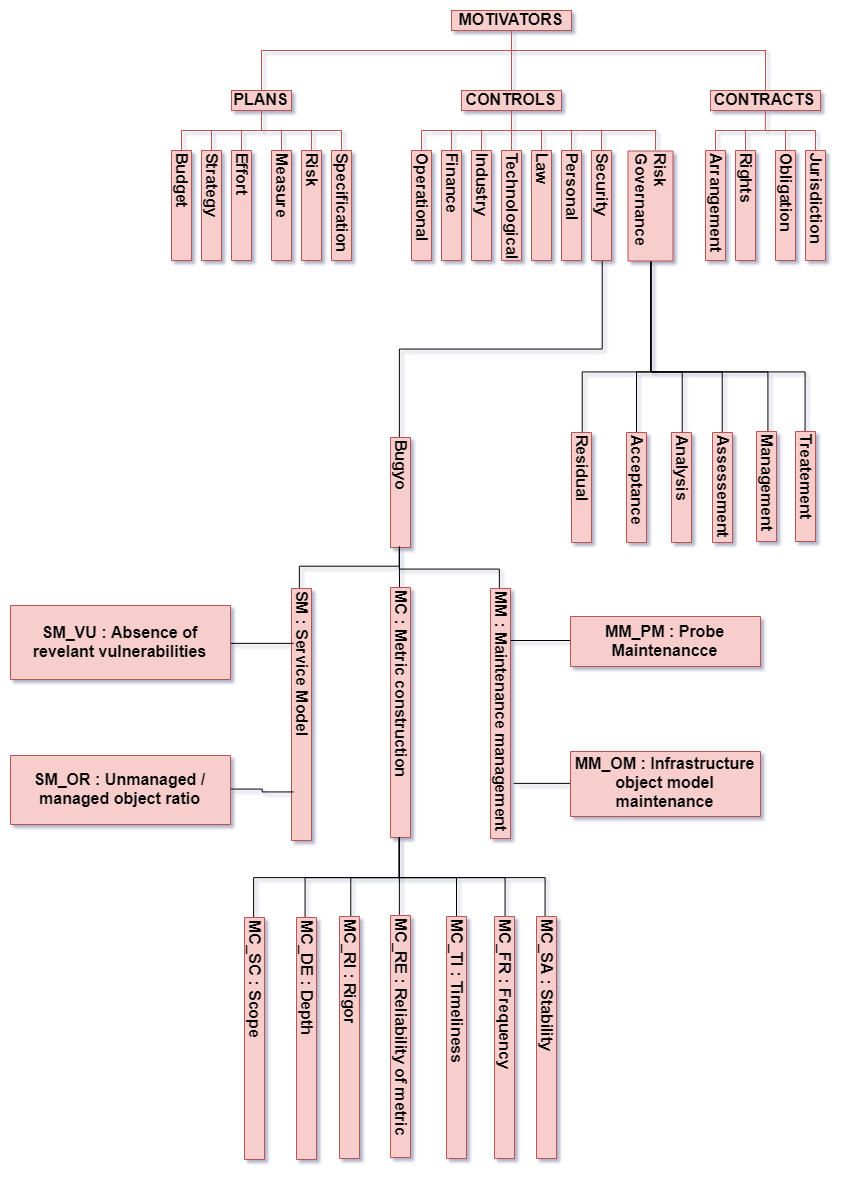
\includegraphics[width=453.75pt,height=632.45pt]{./media/image24.png}
	\end{Center}
\end{figure}


%%%%%%%%%%%%%%%%%%%% Figure/Image No: 17 Ends here %%%%%%%%%%%%%%%%%%%%

%%%%%%%%%%%%%%%%%%%% Biblio %%%%%%%%%%%%%%%%%%%%
\vspace{\baselineskip}
\setlength{\parskip}{8.04pt}
\section*{Bibliograph : }
\addcontentsline{toc}{section}{Bibliograph : }
\textbf{[Web] https ://www.misp-project.org.}\par
\textbf{[Mr Djamel KHADRAOUI, ] Mr Djamel KHADRAOUI. cours Bugyo.}\par
\textbf{[Chris Barden and Amy Lofton and Aubrey Hale and Jenny Ammerman and Claudette Lloyd, 2015]
Chris Barden and Amy Lofton and Aubrey Hale and Jenny Ammerman and Claudette Lloyd (2015).
Amassing a Practical Enterprise Taxonomy. In ARMA Houston Spring Conference.}\par
\textbf{[Abhishek Kumar, 2014] Abhishek Kumar (september 2014). Architecting an Enterprise Content Management Strategy : A Four-Pillar Approach.}\par
\textbf{[A Presentation to Calgary ARMA, 2007]  A Presentation to Calgary ARMA (April 2007).  Functional Classification & Taxonomies.}\par
\textbf{[The World Bank IBRD IDA, 2016] The World Bank IBRD IDA (2016). Sector Taxonomy and definitions.}\par
\textbf{[Web] Taxonomy Code Mapping.}\par
\textbf{[G. Gaupin and H. Knöpfel and P. Morris and E. Motzel and O. Pannenbäcker, 1999] G. Gaupin and H.
Knöpfel and P. Morris and E. Motzel and O. Pannenbäcker (1999). ICB.}\par
\textbf{[The Department of Internal Affairs, 2015] by the Department of Internal Affairs, P. (2015). GEA-NZ
v3.1 Business Reference Model and Taxonomy.}\par
\textbf{[Nezlek, 2015] Nezlek, J. (2015). An Introduction to Multilevel Modeling - basic terms and research
examples.}\par
\textbf{[Web] https ://en.wikipedia.org/wiki/K-means.}\par
\textbf{[Mr Blansche, 2019] Blansche, A. (2019). M1 AI Course 04 / data search course 05 }\par
\textbf{[Web] https ://en.wikipedia.org/wiki/UPGMA.}\par
\textbf{[S. Garcia-Vallve, J. Palau and A. Romeu, 1999] S. Garcia-Vallve, J. Palau and A. Romeu (1999). Horizontal
gene transfer in glycosyl hydrolases inferred from codon usage in Escherichia coli and Bacillus
subtilis. Molecular Biology and Evolution 16(9) :1125-1134.}\par


\printbibliography
\end{document}